\subsection{Hardware Setup}
The breadboard can be divided into 5 segments.  In each of the green segements, the pins are internally connected so as to have the same voltage.  Similarly, in the central segments, the pins in each column  are internally connected in the same fashion as the blue columns. 

\begin{problem}
	Plug the display to the breadboard in Fig. \ref{fig:breadboard}
\end{problem}
\begin{figure}[!h]
\begin{center}
\includegraphics[width=\columnwidth]{./figs/breadboard}
\end{center}
\caption{}
\label{fig:breadboard}
\end{figure}

The seven segment display in Fig. \ref{fig:sevenseg} has eight pins, $a, b, c, d, e, f, g$ and $dot$ that take an active LOW input, i.e.  the LED will glow only if the input is connected to ground.  Each of these pins is connected to an LED segment.  The $dot$ pin is  reserved for the $\cdot$ LED.  

%
%\begin{center}
	%\includegraphics[scale=1]{sevenseg}
%\end{center}

\begin{problem}
	Connect one end of the resistor to the COM pin of the display and the other end to an extreme pin of the breadboard.	
\end{problem}
%
%
%
\begin{figure}[!h]
\begin{center}
\resizebox {0.5\columnwidth} {!} {
\input{./figs/sevenseg.tex}
}
\end{center}
\caption{}
\label{fig:sevenseg}
\end{figure}

The Arduino Uno has some ground pins, analog input pins A0-A3 and digital pins D1-D13 that can be used for both input as well as output. It also has two power pins that can generate 3.3$V$ and 5$V$.  In the following exercises, only the GND, 5$V$ and digital pins will be used.
%
%\begin{center}
	%\includegraphics[scale=1]{arduino}
%\end{center}
%
\begin{problem}
	Connect the 5V pin of the arduino to an  extreme pin that is in the same segment as the 1K resistor pin. 
	\end{problem}	
\begin{problem}
	Connect the GND pin of the arduino to the opposite extreme pin of the breadboard
\end{problem}
\begin{problem}
	Connect the Arduino to the computer.
\end{problem}
\begin{problem}
	Connect the \em{dot} pin of the display to a pin in the same segment as the GND pin.  What do you observe?
\end{problem}
\subsection{Software Setup}
\begin{problem}
Install AVRA and AVRDUDE on your Linux system through the following commands
\begin{lstlisting}
sudo apt-get install avra avrdude
%Finding the port

sudo dmesg | grep tty
%The output will be something like
[    6.153362] cdc_acm 1-1.2:1.0: ttyACM0: USB ACM device
%and your port number is ttyACM0
\end{lstlisting}
\end{problem}
\begin{problem}
Download the m328Pdef.inc file from 
\begin{lstlisting}
http://tlc.iith.ac.in/img/m328Pdef.inc
\end{lstlisting}
%\lstinputlisting[language=C]{./codes/setup/incfile.tex}
and copy into the directory home (/home/user/) directory
\end{problem}
%
\begin{problem}
Open \textbf{geany} and type the following code.  Save the file as \textbf{hello.asm}
\end{problem}
\lstinputlisting[language=C]{./codes/hello/hello.asm}
\begin{problem}
With \textbf{hello.asm} open in \textbf{geany}, go to Build$\rightarrow$Set Build Commands$\rightarrow$Compile and enter 
\begin{lstlisting}
avra "%f"
\end{lstlisting}
%
Then  go to Build$\rightarrow$Set Build Commands$\rightarrow$Execute and enter
\begin{lstlisting}
avrdude -p atmega328p -c arduino -P /dev/ttyACM0 -b 115200 -U flash:w:%e.hex
\end{lstlisting}
\end{problem}
%
\begin{problem}
Change \textbf{/home/linaro/m328Pdef.inc} in \textbf{hello.asm} to \textbf{/home/username/m328Pdef.inc}, where
{\em username} is your linux login name.
\end{problem}
\subsection{Controlling the Display}
\begin{problem}
Now connect the dot pin of the display to pin 13 of the arduino.  Use \textbf{F8} to compile \textbf{hello.asm}
and \textbf{F5} to execute.
\end{problem}

\begin{problem}
Turn the LED off by modifying \textbf{hello.asm.}
\end{problem}

%
\begin{problem}
Complete   Table \ref{table:pinmap} 
for all the digital pins using Fig. \ref{fig:Atmega168PinMap2}
\end{problem}
%
\input{./figs/pinmap.tex}
\begin{figure}[!h]
\begin{center}
\includegraphics[width=\columnwidth]{./figs/Atmega168PinMap2}
\end{center}
\caption{}
\label{fig:Atmega168PinMap2}
\end{figure}
%
\begin{problem}
\label{prob:disp}
Connect the $a-g$ pins of the display to the 2-8 pins of the arduino.  Run the following code.
\lstinputlisting[language=C]{./codes/sevenseg/sevenseg.asm}
\end{problem}
%
\begin{problem}
The output of Problem \ref{prob:disp} can be explained by Table \ref{table:ass_arduinoport} below. 	Complete Table \ref{table:ass_arduinoport} for all numbers between 0-9.
Use this information to display the numbers from 0-9 .
\input{./figs/ass_arduinoport}
%\input{./figs/arduinoport}
\end{problem}
%\begin{problem}
%	Complete Table \ref{table:ass_arduinoport} for all numbers between 0-9.
%\end{problem}
%%
%\begin{problem}
%	Now generate the numbers from 1-9 on the display using Table \ref{table:ass_arduinoport}.
%\end{problem}
%%
%The 7447 IC helps in displaying decimal numbers on the seven segment display.  The $\bar{a}-\bar{f}$, pins of the 7447 IC are connected to the $a-f$ pins of the display. $V_{cc}$ should be connected to a 5V power source. The input pins of the decoder are A,B,C and D, with A being the lowest significant bit (LSB) and D being the most significant bit (MSB).  For example, the number 5 is visible on the display when the A,B,C and D inputs are the following.
%\begin{center}
%	\begin{tabular}{|c|c|c|c|c|}
%\hline
%D & C & B & A & Decimal
%\\ \hline
%0 & 1 & 0 & 1 & 5
%\\
%\hline
%\end{tabular}
%\end{center}
%
%%
%\begin{figure}[!h]
%\begin{center}
%\includegraphics[width=\columnwidth]{./figs/7447IC}
%\end{center}
%\caption{}
%\label{}
%\end{figure}
%
%%\begin{center}
%	%\includegraphics[scale=1.5]{7447IC}
%%\end{center}
%
%%
%\begin{problem}
%	Connect the 7447 IC decoder $\bar{a}-\bar{g}$ pins to the $a-g$ pins of the display respectively.
%\end{problem}
%\begin{problem}
%	Connect the $V_{cc}$ and GND pins of the decoder to the 5V supply and GND pins of the breadboard.
%\end{problem}
%\begin{problem}
%	Connect the A,B,C,D pins to pins in the GND extreme segment of the breadboard.  What do you observe.
%\end{problem}
%\begin{problem}
%	Now remove the D pin from the breadboard and observe the display output.
%\end{problem}
%\begin{problem}
%	Generate a table with A,B,C,D inputs and the equivalent decimal number output.
%\end{problem}
